\section{Graph databases}

Relational databases often struggle with efficiently managing and querying complex relationships between data entities. 
In contrast, graph databases are specifically designed to handle such tasks using graph structures, which consist of nodes (entities), edges (relationships), and properties (data about the entities or relationships).
Key features of graph databases include:
\begin{itemize}
    \item \textit{Index-free adjacency}: each node directly references its adjacent nodes, eliminating the need for costly index lookups during traversal.
    \item \textit{Relationships as first-class citizens}: in graph databases, edges, or relationships, carry much of the critical information. 
\end{itemize}
They not only connect nodes to other nodes but can also link nodes to properties, making the data structure highly flexible for relationship-focused queries.
Graph databases excel when working with datasets that are rich in relationships, making them an ideal fit for scenarios where relationships are central to the analysis:
\begin{itemize}
    \item \textit{High performance on relationship queries}: graph databases are optimized for associative datasets, such as social networks, where the relationships between entities are as important as the entities themselves.
    \item \textit{Natural fit for object-oriented models}: graph databases map more intuitively to object-oriented applications, as they inherently support hierarchical structures like parent-child relationships and object classification.
    \item \textit{Efficient traversal}: because nodes directly point to adjacent nodes, queries that involve traversing relationships, such as finding paths or analyzing networks, are much faster compared to relational databases.
\end{itemize}
One significant challenge with graph databases is that the complexity of the data model can escalate rapidly, leading to maintainability issues. 
As relationships grow in number and intricacy, managing the graph can become increasingly difficult.

Additionally, performing queries on graph databases can be complex. 
Crafting efficient queries often requires a deep understanding of the graph structure and the relationships between nodes, which can complicate both development and performance optimization.
To simplify the quering process we run a graph matching approach (pattern matching)

\subsection{Neo4j}
Neo4j, developed by Neo Technologies, is the most popular graph database available today. 
It is implemented in Java and is open-source, making it accessible for various applications.
The key features of Neo4j are: 
\begin{itemize}
    \item \textit{Schema-free}: Neo4j allows for a flexible data model where data does not need to conform to a specific schema, facilitating easier updates and modifications.
    \item \textit{ACID compliance}: it ensures atomicity, consistency, isolation, and durability for logical units of work, which is crucial for maintaining data integrity.
    \item \textit{User-friendly}: Neo4j is designed to be easy to get started with and use, providing a smooth onboarding experience for new users.
    \item \textit{Extensive documentation and community}: it boasts thorough documentation and a large, active developer community, making it easier to find support and resources.
    \item \textit{Multi-language support}: Neo4j supports a wide range of programming languages, including Java, Python, Perl, Scala, and its own query language, Cypher.
\end{itemize}
\begin{figure}[H]
    \centering
    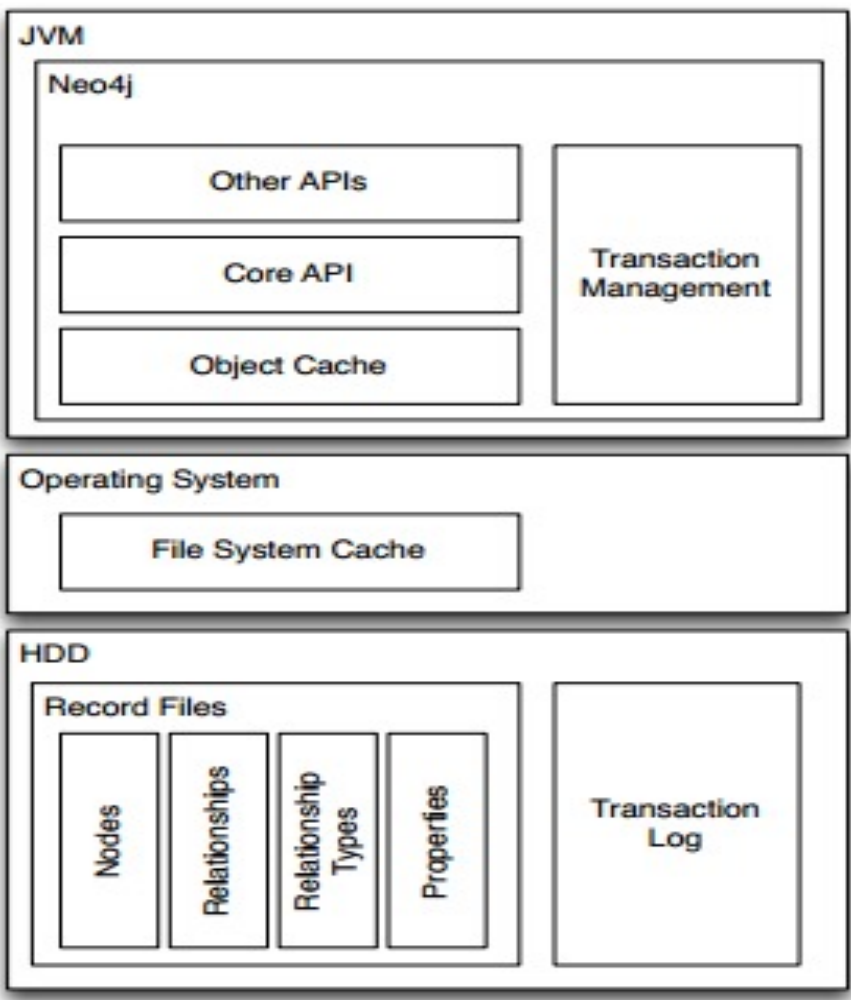
\includegraphics[width=0.75\linewidth]{images/neo4j.png}
    \caption{Neo4j architecture}
\end{figure}
Neo4j is primarily intended as an operational database rather than a dedicated analytics platform.
It excels in managing relationships and efficiently accessing nodes, although it may not be as effective for comprehensive graph-wide analyses.

\subsection{Data model}
Neo4j is based on: 
\begin{itemize}
    \item \textit{Nodes}: represent entities, equipped with labels (types) and attributes (properties).
    \item \textit{Edges}: serve as the connections between nodes, providing context and relationships.
    \item \textit{Indexes}: enhance query performance by allowing quick lookups of nodes and relationships.
\end{itemize}

\subsection{Query language}
Cypher is the dedicated query language for Neo4j, designed to be both user-friendly and powerful. 
Its declarative nature allows users to specify what data they want to retrieve without needing to define how to obtain it, making query formulation straightforward.
One of the standout features of Cypher is its emphasis on relationships, which enables users to easily navigate and manipulate complex graph structures. 
This relationship-centric approach simplifies the querying process compared to traditional SQL, where handling joins can become cumbersome and complex.
Many of Cypher's capabilities have been specifically developed to address common challenges faced with SQL, enhancing its usability and efficiency in dealing with graph data. 

The Cypher query language in Neo4j supports several key operations for managing and querying graph data. 
Below is an overview of the primary operations:
\begin{itemize}
    \item \textit{Data creation}: to create new nodes and relationships in Neo4j, Cypher provides the \texttt{CREATE} command.
        \begin{verbatim}
CREATE (n:Label {propertyKey: value, ... })
        \end{verbatim}
        To create a new relationship we write: 
        \begin{verbatim}
CREATE (n1)-[r:RELATIONSHIP_TYPE {propertyKey: value, ...}]->(n2)
        \end{verbatim}
        Note that a node may have two labels: 
        \begin{verbatim}
CREATE (n:Label1:Label2 {propertyKey: value, ... })
        \end{verbatim}
    \item \textit{Data importing}: we can aslo import an entire graph from a csv file in the following way: 
        \begin{verbatim}
USING PERIODIC COMMIT 
LOAD CSV WITH HEADERS FROM "file:customers.csv" AS row
CREATE (:Customer {companyName: row.CompanyName, ID: row.CustomerID}); 
        \end{verbatim}
        The periodic commit is used to guarantee the ACID properties. 
    \item \textit{Data merging}: To ensure you don't create duplicate nodes or relationships, use the merge operation: 
        \begin{verbatim}
MERGE (p:Person {name: 'John Doe'})
ON CREATE SET p.age = 30
ON MATCH SET p.lastUpdated = date()  
        \end{verbatim}
        We can also merge edges in the same way, avoiding duplicates. 
    \item \textit{Index creation}: create an index over a certain data type: 
        \begin{verbatim}
CREATE INDEX ON :Customer(customerID);
        \end{verbatim}
    \item \textit{Constraints creation}: create a constraint over a certain data type: 
        \begin{verbatim}
CREATE CONSTRAINT ON (c:Customer)
ASSERT c.customerID IS UNIQUE;
        \end{verbatim}
    \item \textit{Data querying}: the general query in Cypher is: 
        \begin{verbatim}
MATCH (user)-[:FRIEND]-(friend)
WITH user, count(friend) AS friends
ORDER BY friends DESC
SKIP 1 LIMIT 3
RETURN user
        \end{verbatim}
        Aggregation can be used (\texttt{COUNT}).
        \texttt{WITH} separates query parts explicitly, to declare the variables for the next part.
        \texttt{SKIP} skips results at the top and \texttt{LIMIT} limits the number of results.
        We can also add an \texttt{*} to a relationship to find all the nodes not directly connected. 
\end{itemize}